%% LyX 2.0.3 created this file.  For more info, see http://www.lyx.org/.
%% Do not edit unless you really know what you are doing.
\documentclass[twoside,english]{paper}
\usepackage{lmodern}
\renewcommand{\ttdefault}{lmodern}
\usepackage[T1]{fontenc}
\usepackage[latin9]{inputenc}
\usepackage[a4paper]{geometry}
\geometry{verbose,tmargin=3cm,bmargin=2.5cm,lmargin=2cm,rmargin=2cm}
\usepackage{color}
\usepackage{babel}
\usepackage{float}
\usepackage{bm}
\usepackage{amsthm}
\usepackage{amsmath}
\usepackage{amssymb}
\usepackage{graphicx}
\usepackage{esint}
\usepackage[unicode=true,pdfusetitle,
 bookmarks=true,bookmarksnumbered=false,bookmarksopen=false,
 breaklinks=false,pdfborder={0 0 0},backref=false,colorlinks=false]
 {hyperref}
\usepackage{breakurl}
\usepackage{makeidx}

\makeatletter

%%%%%%%%%%%%%%%%%%%%%%%%%%%%%% LyX specific LaTeX commands.
%% Because html converters don't know tabularnewline
\providecommand{\tabularnewline}{\\}

%%%%%%%%%%%%%%%%%%%%%%%%%%%%%% Textclass specific LaTeX commands.
\numberwithin{equation}{section}
\numberwithin{figure}{section}

%%%%%%%%%%%%%%%%%%%%%%%%%%%%%% User specified LaTeX commands.
\usepackage{babel}

\@ifundefined{showcaptionsetup}{}{%
 \PassOptionsToPackage{caption=false}{subfig}}
\usepackage{subfig}
\makeatother

\usepackage{listings}


\begin{document}

\title{Generalised parton distributions}

\author{Valerio Bertone}

\tableofcontents{}

\section{Introduction}

In this set of notes I collect the technical aspects concerning
generalised parton distributions (GPDs). Since the computation GPDs
introduces new kinds of convolution integrals, a strategy aimed at
optimising the numerics needs to be devised.

\section{Evolution equation}

In general, the evolution equation for GPDs reads:
\begin{equation}\label{eq:eveq}
\mu^2\frac{d}{d\mu^2}f(x,\xi) = \int_{-\infty}^{+\infty}\frac{dx'}{\left|2\xi\right|}P\left(\frac{x}{\xi},\frac{x'}{\xi}\right)f(x',\xi)\,.
\end{equation}
The GPD $f$ and the evolution kernel $P$ may in general be a vector
and a matrix in flavour space. For now we will just be concerned with
the integral in the r.h.s. of Eq.~(\ref{eq:eveq}) regardless of the
flavour structure. The support of the evolution kernel
$P\left(\frac{x}{\xi},\frac{x'}{\xi}\right)$ is shown in
Fig.~\ref{fig:GPDIntDomain}.
\begin{figure}[h]
  \begin{centering}
    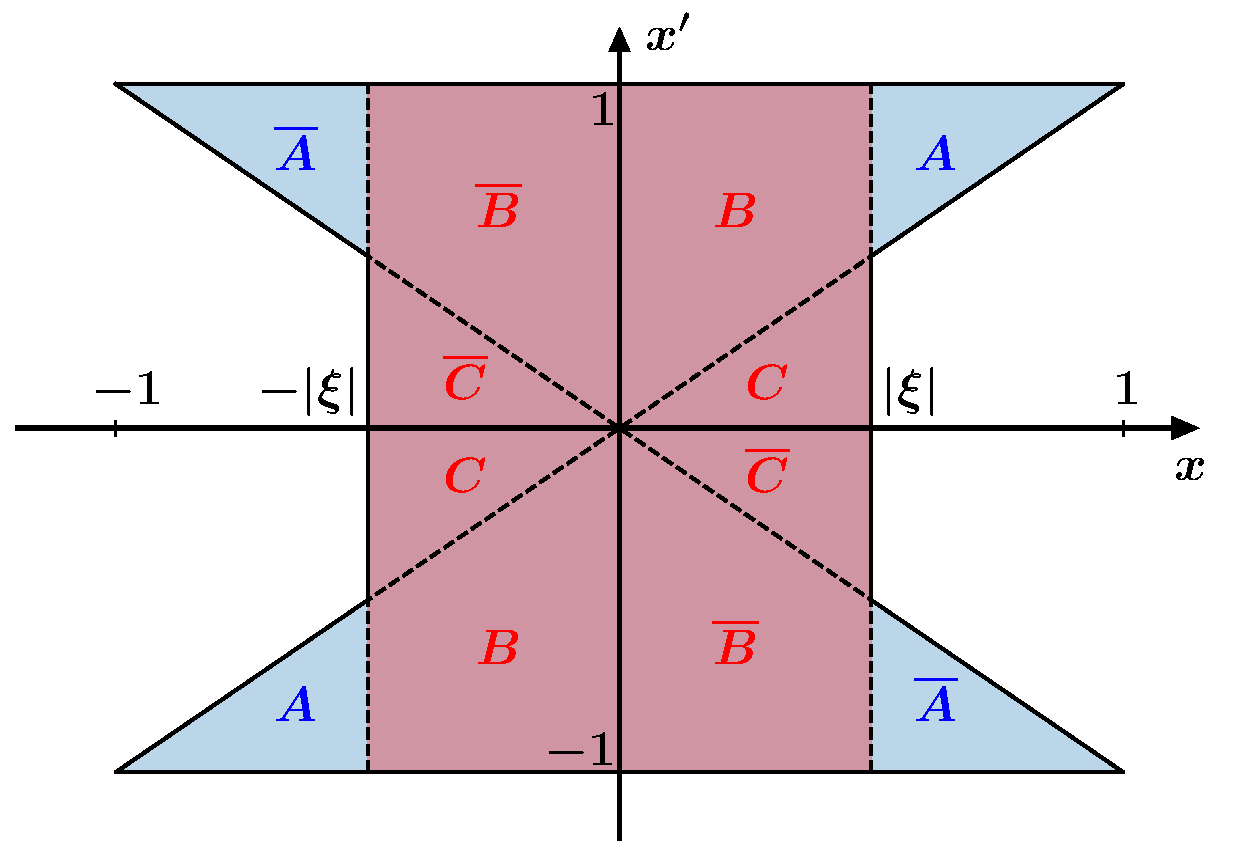
\includegraphics[width=0.7\textwidth]{plots/GPDIntDomain}
    \caption{Support domain of the evolution kernel
      $P\left(\frac{x}{\xi},\frac{x'}{\xi}\right)$.\label{fig:GPDIntDomain}}
  \end{centering}
\end{figure}
Knowing the support of the evolution kernel, Eq.~(\ref{eq:eveq}) can
be rearranged as follows:
\begin{equation}
\displaystyle\mu^2\frac{d}{d\mu^2}f(\pm x,\xi) =\int_{b(x)}^{1}\frac{dx'}{x'}\left[\frac{x'}{\left|2\xi\right|}P\left(\pm \frac{x}{\xi},\frac{x'}{\xi}\right)f(x',\xi)+\frac{x'}{\left|2\xi\right|}P\left(\mp \frac{x}{\xi},\frac{x'}{\xi}\right)f(-x',\xi)\right]\,,
\end{equation}
with:
\begin{equation}\label{eq:lowintb}
b(x) = |x|\theta\left(\left|\frac{x}{\xi}\right|-1\right)\,,
\end{equation}
and where we have used the symmetry property of the evolution kernels
$P(y,y')=P(-y,-y')$. In the unpolarised case, it is useful to
define:\footnote{Notice the seemingly unusual fact that $f^{+}$ is
  defined as difference and $f^{-}$ as sum of GPDs computed at
  opposite values of $x$. This can be understood from the fact that,
  in the forward limit, $f(-x)= -\overline{f}(x)$, \textit{i.e.} the
  PDF of a quark computed at $-x$ equals the PDF of the corresponding
  antiquark computed at $x$ with opposite sign.}
\begin{equation}\label{eq:pmdef}
\begin{array}{rcl}
\displaystyle f^{\pm}(x,\xi) &=&\displaystyle  f(x,\xi) \mp
                       f(-x,\xi)\,,\\
\\
\displaystyle P^{\pm}(y,y') &=&\displaystyle  P(y,y') \mp P(-y,y')\,,
\end{array}
\end{equation}
so that the evolution equation for $f^{\pm}$ reads:
\begin{equation}\label{eq:eveq2}
\displaystyle\mu^2\frac{d}{d\mu^2}f^{\pm}(x,\xi) = \int_{b(x)}^{1}\frac{dx'}{x'}\frac{x'}{\left|2\xi\right|}
                                                         P^{\pm}\left(\frac{x}{\xi},\frac{x'}{\xi}\right)f^{\pm}(x',\xi)\,.
\end{equation}
It is relevant to observe that the presence of the $\theta$-function
in the lower integration bound $b$, Eq.~(\ref{eq:lowintb}), is such
that for $|x|>|\xi|$ the evolution equation has the exact form of the
DGLAP evolution equation which corresponds to integrating over the
blue regions in Fig.~\ref{fig:GPDIntDomain} (henceforth DGLAP
region). Conversely, for $|x|\leq|\xi|$ the lower integration bound
becomes zero and the evolution equation assumes the form of the
so-called ERBL equation that describes the evolution of meson
distribution amplitudes (DAs). This corresponds to integrating over
the red region (henceforth ERBL region). Crucially, in the limits
$\xi\rightarrow 0$ and $\xi\rightarrow \pm1$ one recovers the DGLAP
and ERBL equations, respectively.

For later convenience, we define the parameter:
\begin{equation}
\kappa(x) = \frac{\xi}{x}\,,
\end{equation}
so that:
\begin{equation}
\frac{x'}{\left|2\xi\right|}
P^{\pm}\left(\frac{x}{\xi},\frac{x'}{\xi}\right)=\frac{1}{2\kappa}
\frac{x'}{x} P^{\pm}\left(\frac{1}{\kappa},\frac{1}{\kappa}
  \frac{x'}{x}\right)\equiv \mathcal{P}^{\pm}\left(\kappa,\frac{x}{x'}\right)\,,
\end{equation}
where the last equality effectively defines the \textit{DGLAP-like}
splitting function:
\begin{equation}\label{eq:DGLAPevk}
\mathcal{P}^{\pm}(\kappa,y) = \frac{1}{2\kappa y}
P^{\pm}\left(\frac{1}{\kappa},\frac{1}{\kappa y}\right)\,.
\end{equation}
Plugging this definition into the integral in the r.h.s. of
Eq.~(\ref{eq:eveq2}) and performing a change of variable gives:
\begin{equation}\label{eq:DGLAPforGPDs}
\displaystyle\mu^2\frac{d}{d\mu^2}f^{\pm}(x,\xi)= \int_{x}^{x/b(x)}\frac{dy}{y}\mathcal{P}^{\pm}\left(\kappa,y\right)f^{\pm}\left(\frac{x}{y},\xi\right)\,,
\end{equation}
which (almost) has the form of a ``standard'' DGLAP equation. The only
difference is that the upper integration bound is not one but rather
$x/b(x)$ with $b(x)$ defined in Eq.~(\ref{eq:lowintb}). As discussed
in the document \textit{IntegralStructure.pdf}, this difference can be
handled within APFEL (up to a numerical approximation to be assessed)
by adjusting the integration procedure.

A crucial ingredient for an efficient implementation of GPD evolution
is the availability of the DGLAP-like splitting functions
$\mathcal{P}^{\pm}$ defined in Eq.~(\ref{eq:DGLAPevk}) in a closed
form amenable to be easily integrated as in
Eq.~(\ref{eq:DGLAPforGPDs}).

\subsection{On continuity of GPDs}

It is well known that GPDs are required to be continuous at $x=\xi$
for factorisation to be valid~\cite{Radyushkin:1997ki}. It is thus
interesting to consider the consequence of this constraint. To this
end, let us consider the limits of Eq.~(\ref{eq:eveq2}) for
$x\rightarrow \xi^\pm$:
\begin{equation}\label{eq:limit1}
\lim_{x\rightarrow \xi^+}\displaystyle\mu^2\frac{d}{d\mu^2}f^{\pm}(x,\xi) = \mu^2\frac{d}{d\mu^2}f^{\pm}(\xi,\xi)=\int_{\xi}^{1}\frac{dx'}{\left|2\xi\right|}
                                                         P^{\pm}\left(\frac{\xi^+}{\xi},\frac{x'}{\xi}\right)f^{\pm}(x',\xi)\,,
\end{equation}
and:
\begin{equation}\label{eq:limit2}
\lim_{x\rightarrow \xi^-}\displaystyle\mu^2\frac{d}{d\mu^2}f^{\pm}(x,\xi) = \mu^2\frac{d}{d\mu^2}f^{\pm}(\xi,\xi)=\int_{0}^{1}\frac{dx'}{\left|2\xi\right|}
                                                         P^{\pm}\left(\frac{\xi^-}{\xi},\frac{x'}{\xi}\right)f^{\pm}(x',\xi)\,,
\end{equation}
where we have used the continuity of $f^{\rm}$ at $x=\xi$. For the
non-singlet anomalous dimension at one loop, one can easily verify
that:
\begin{equation}
  P^{\pm}\left(\frac{\xi^+}{\xi},y\right) =
  P^{\pm}\left(\frac{\xi^-}{\xi},y\right) = P^{\pm}\left(1,y\right)\,.
\end{equation}
Taking the difference between Eqs.~(\ref{eq:limit1})
and~(\ref{eq:limit2}), one finds, at least for a non-singlet
distribution at one loop, that:
\begin{equation}
\int_{0}^{\xi}dx'\,P^{\pm}\left(1,\frac{x'}{\xi}\right)f^{\pm}(x',\xi)=0\,.
\end{equation}
This appears to be some sort of (valence) sum rule that the GPDs have
to fulfil.

% \section{Treatment of the plus prescription}

% In the case of the evolution of GPDs we deal with complicated
% evolution kernels whose algebraic structure is hard to
% disentangle. Therefore, we need to devise a general strategy to treat
% the plus prescriptions that arise for the cancellation of soft gluons
% in order to make them easily implementable. The case to treat is
% function of this kind:
% \begin{equation}
% P(y) = \left[\frac{F(y)}{1-y}\right]_+\,,
% \end{equation}
% where $F(y)$ is a regular function at $y=1$. The first step is to
% write this function as follows:
% \begin{equation}
% P(y) = R(y)+S\left(\frac1{1-y}\right)_++L\delta(1-y)\,,
% \end{equation}
% where $R(y)$ is a regular function at $y=1$, and $S$ and $L$ are
% constants that need to be determined. To this end we compute the
% integral:
% \begin{equation}
% I=\int_0^1dy\,P(y)f(y)\,,
% \end{equation}
% where $f(y)$ is a regular function at $y=1$. Using the definition of
% plus distribution, we find:
% \begin{equation}\label{eq:intstep}
% \begin{array}{rcl}
% I&=&\displaystyle\int_0^1dy\,\frac{F(y)}{1-y}\left[f(y)-f(1)\right]=\int_0^1dy\,\frac{1}{1-y}\left[F(y)
%   f(y)-F(y) f(1)-F(1)f(1)+F(1)f(1)\right]\\
% \\
% &=&\displaystyle\int_0^1dy\,\frac{F(y)}{\left(1-y\right)_+}f(y)-f(1)\int_0^1dz\,\frac{F(z)}{\left(1-z\right)_+}=\int_0^1dy\,\left[\frac{F(y)}{\left(1-y\right)_+}+L\delta(1-y)\right]f(y)\,,
% \end{array}
% \end{equation}
% where in the last step we have defined:
% \begin{equation}
% L=-\int_0^1dz\,\frac{F(z)}{\left(1-z\right)_+}=-\int_0^1dz\,\frac{F(z)-F(1)}{1-z}\,.
% \end{equation}
% In order to find $R$ and $S$, we just rewrite the last step of
% Eq.~(\ref{eq:intstep}) as:
% \begin{equation}
% I=\int_0^1dy\,\left[\frac{F(y)-F(1)}{1-y}+F(1)\left(\frac{1}{1-y}\right)_++L\delta(1-y)\right]f(y)\,,
% \end{equation}
% that allows us to read off:
% \begin{equation}
%  S = F(1) \,,\qquad R(y)=\frac{F(y)-S}{1-y}\,,\qquad L = -\int_0^1dy\,R(y)\,.
% \end{equation}
% For an incomplete integral between $x$ and one, typical of a Mellin
% convolution, the result is:
% \begin{equation}
% I(x)=\int_x^1dy\,\left[\frac{F(y)-S}{1-y}+S\left(\frac{1}{1-y}\right)_++\left(L+S\ln(1-x)\right)\delta(1-y)\right]f(y)\,.
% \end{equation}

% \section{Flavour structure}

% In this section we report the leading-order (LO) evolution kernels
% $\mathcal{P}^\pm$ taking into the flavour structure. The explicit
% expressions of the relevant LO kernels are extracted from
% Ref.~\cite{Blumlein:1999sc}. As usual, the perturbative expansion of
% the evolution kernels reads:
% \begin{equation}
%   \mathcal{P}^{\pm}(\kappa,y;\mu) = \sum_{n=0}^\infty \left(\frac{\alpha_s(\mu)}{4\pi}\right)^{n+1}\mathcal{P}^{\pm,[n]} (\kappa,y)\,.
% \end{equation}

% At leading-order (LO) it turns out that the evolution kernels $P$
% appearing in Eq.~(\ref{eq:eveq}) vanish for negative values of
% $x'$. As a consequence of the definition in Eq.~(\ref{eq:pmdef}), at
% LO one has $P^{+}=P^{-}$. The explicit form of the LO evolution
% kernels $\mathcal{P}$, defined in Eq.~(\ref{eq:DGLAPevk}), is:
% \begin{equation}
% \begin{array}{rcl}
% \mathcal{P}_{qq,\rm NS}^{\pm,[0]} (\kappa,y) &=&\displaystyle
%                                                  2C_F\left[\frac{-1-y}{1-\kappa^2
%                                                  y^2}+2\left(\frac{1}{1-y}\right)_+-\left(\frac{(1+\kappa)\ln(1-\kappa)+(1-\kappa)\ln(1+\kappa)}{2\kappa^2}\right)\delta(1-x)\right]\,,\\
% \\
% \mathcal{P}_{qg}^{\pm,[0]} (\kappa,y)  &=&\displaystyle 4n_f T_R\frac{1}{1-\kappa^2y^2}
%                                            \left[1-\frac{2 y(1-y)}{1-\kappa^2
%                                            y^2}\right]\,,\\
% \\
% \mathcal{P}_{gq}^{\pm,[0]} (\kappa,y)  &=&\displaystyle
% 2C_F\left[\frac{(1-y)^2}{y(1-\kappa^2 y^2)}+\frac1y\right]\,,\\
% \\
% \mathcal{P}_{gg}^{\pm,[0]} (\kappa,y) &=&\displaystyle
%                                           4C_A\left[\frac{-2+(1+\kappa^2)y-(1-\kappa^2)y^2}{(1-\kappa^2
%                                           y^2)^2}+\frac{1}{y}+ \left(\frac{1}{1-y}\right)_+\right]+\left(\frac{11}{3}C_A-\frac{4}{3}n_fT_R\right)\delta(1-x)\,.
% \end{array}
% \end{equation}


\newpage

\begin{thebibliography}{alp}

%\cite{Diehl:2003ny}
\bibitem{Diehl:2003ny}
  M.~Diehl,
  %``Generalized parton distributions,''
  Phys.\ Rept.\  {\bf 388} (2003) 41
  doi:10.1016/j.physrep.2003.08.002, 10.3204/DESY-THESIS-2003-018
  [hep-ph/0307382].
  %%CITATION = doi:10.1016/j.physrep.2003.08.002, 10.3204/DESY-THESIS-2003-018;%%
  %1016 citations counted in INSPIRE as of 30 Oct 2019

%\cite{Blumlein:1999sc}
\bibitem{Blumlein:1999sc}
  J.~Blumlein, B.~Geyer and D.~Robaschik,
  %``The Virtual Compton amplitude in the generalized Bjorken region: twist-2 contributions,''
  Nucl.\ Phys.\ B {\bf 560} (1999) 283
  doi:10.1016/S0550-3213(99)00418-6
  [hep-ph/9903520].
  %%CITATION = doi:10.1016/S0550-3213(99)00418-6;%%
  %86 citations counted in INSPIRE as of 13 Feb 2020

%\cite{Radyushkin:1997ki}
\bibitem{Radyushkin:1997ki}
A.~V.~Radyushkin,
%``Nonforward parton distributions,''
Phys. Rev. D \textbf{56} (1997), 5524-5557
doi:10.1103/PhysRevD.56.5524
[arXiv:hep-ph/9704207 [hep-ph]].
%1104 citations counted in INSPIRE as of 02 Jul 2020

\end{thebibliography}




\end{document}
